\documentclass{article}
\usepackage{graphicx}
\usepackage{wrapfig}
\usepackage{subcaption}
\usepackage[margin=1in]{geometry}
\usepackage{amsmath} % or simply amstext
\usepackage{siunitx}
\usepackage{booktabs}
\usepackage[export]{adjustbox}
\newcommand{\angstrom}{\textup{\AA}}
\usepackage{cleveref}
\usepackage{booktabs}
\usepackage{gensymb}
\usepackage{float}

\title{Supplmental Information : Understanding the nanoscale structure of hexagonal phase lyotropic liquid crystal membranes}
\author{Benjamin J. Coscia \and Douglas L. Gin \and Richard D. Noble \and Joe Yelk \and Matthew Glaser \and Xunda Feng \and Michael R. Shirts}

\begin{document}

\graphicspath{{./figures/}}  % put all the figures here
\maketitle

\begin{wrapfigure}{R}{0.4\textwidth}
      \centering
      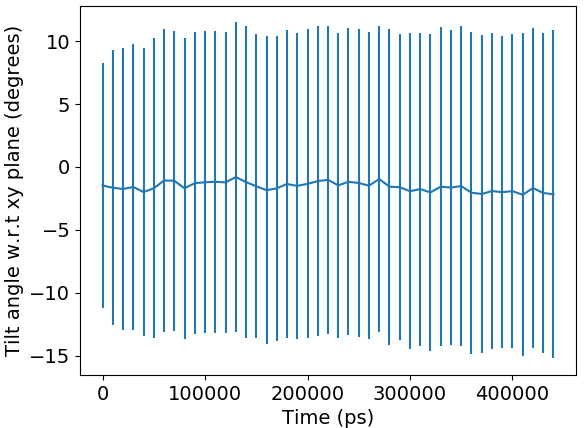
\includegraphics[width=0.4\textwidth]{tilt.png}
      \caption{The average angle between alkane chains and the xy plane is nearly zero degrees}\label{fig:tilt}     
\end{wrapfigure}


\begin{figure}
	\centering
	\begin{subfigure}{0.45\textwidth}
		\centering
		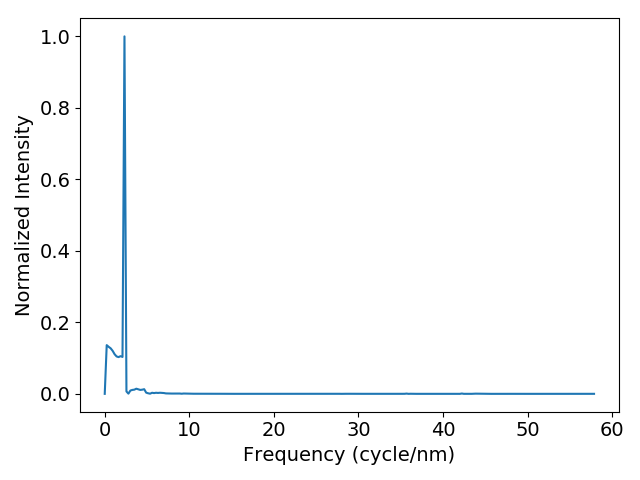
\includegraphics[width=\textwidth]{ps5layered.png}
		\caption{}\label(fig:ps5layered}
	\end{subfigure}
	\begin{subfigure}
		\centering
		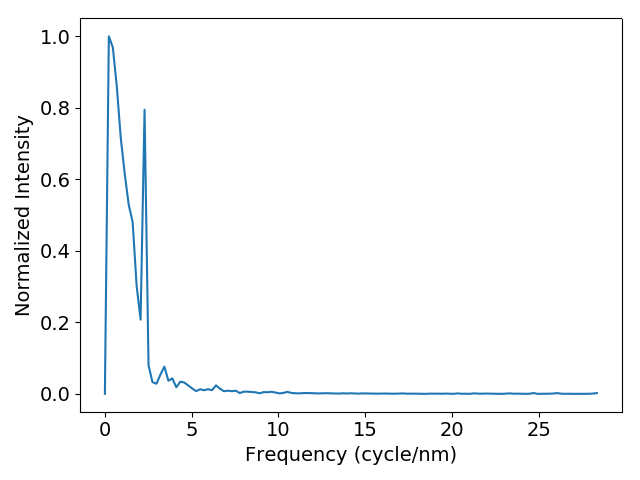
\includegraphics[width=\textwidth]{ps5offset.png}
		\caption{}\label{fig:ps5offset}
	\end{subfigure}
\end{figure}


\begin{figure}[!ht]
        \centering
        \begin{subfigure}{0.45\textwidth}
                \centering
                \hspace{-1cm}
                \vspace{1cm}
                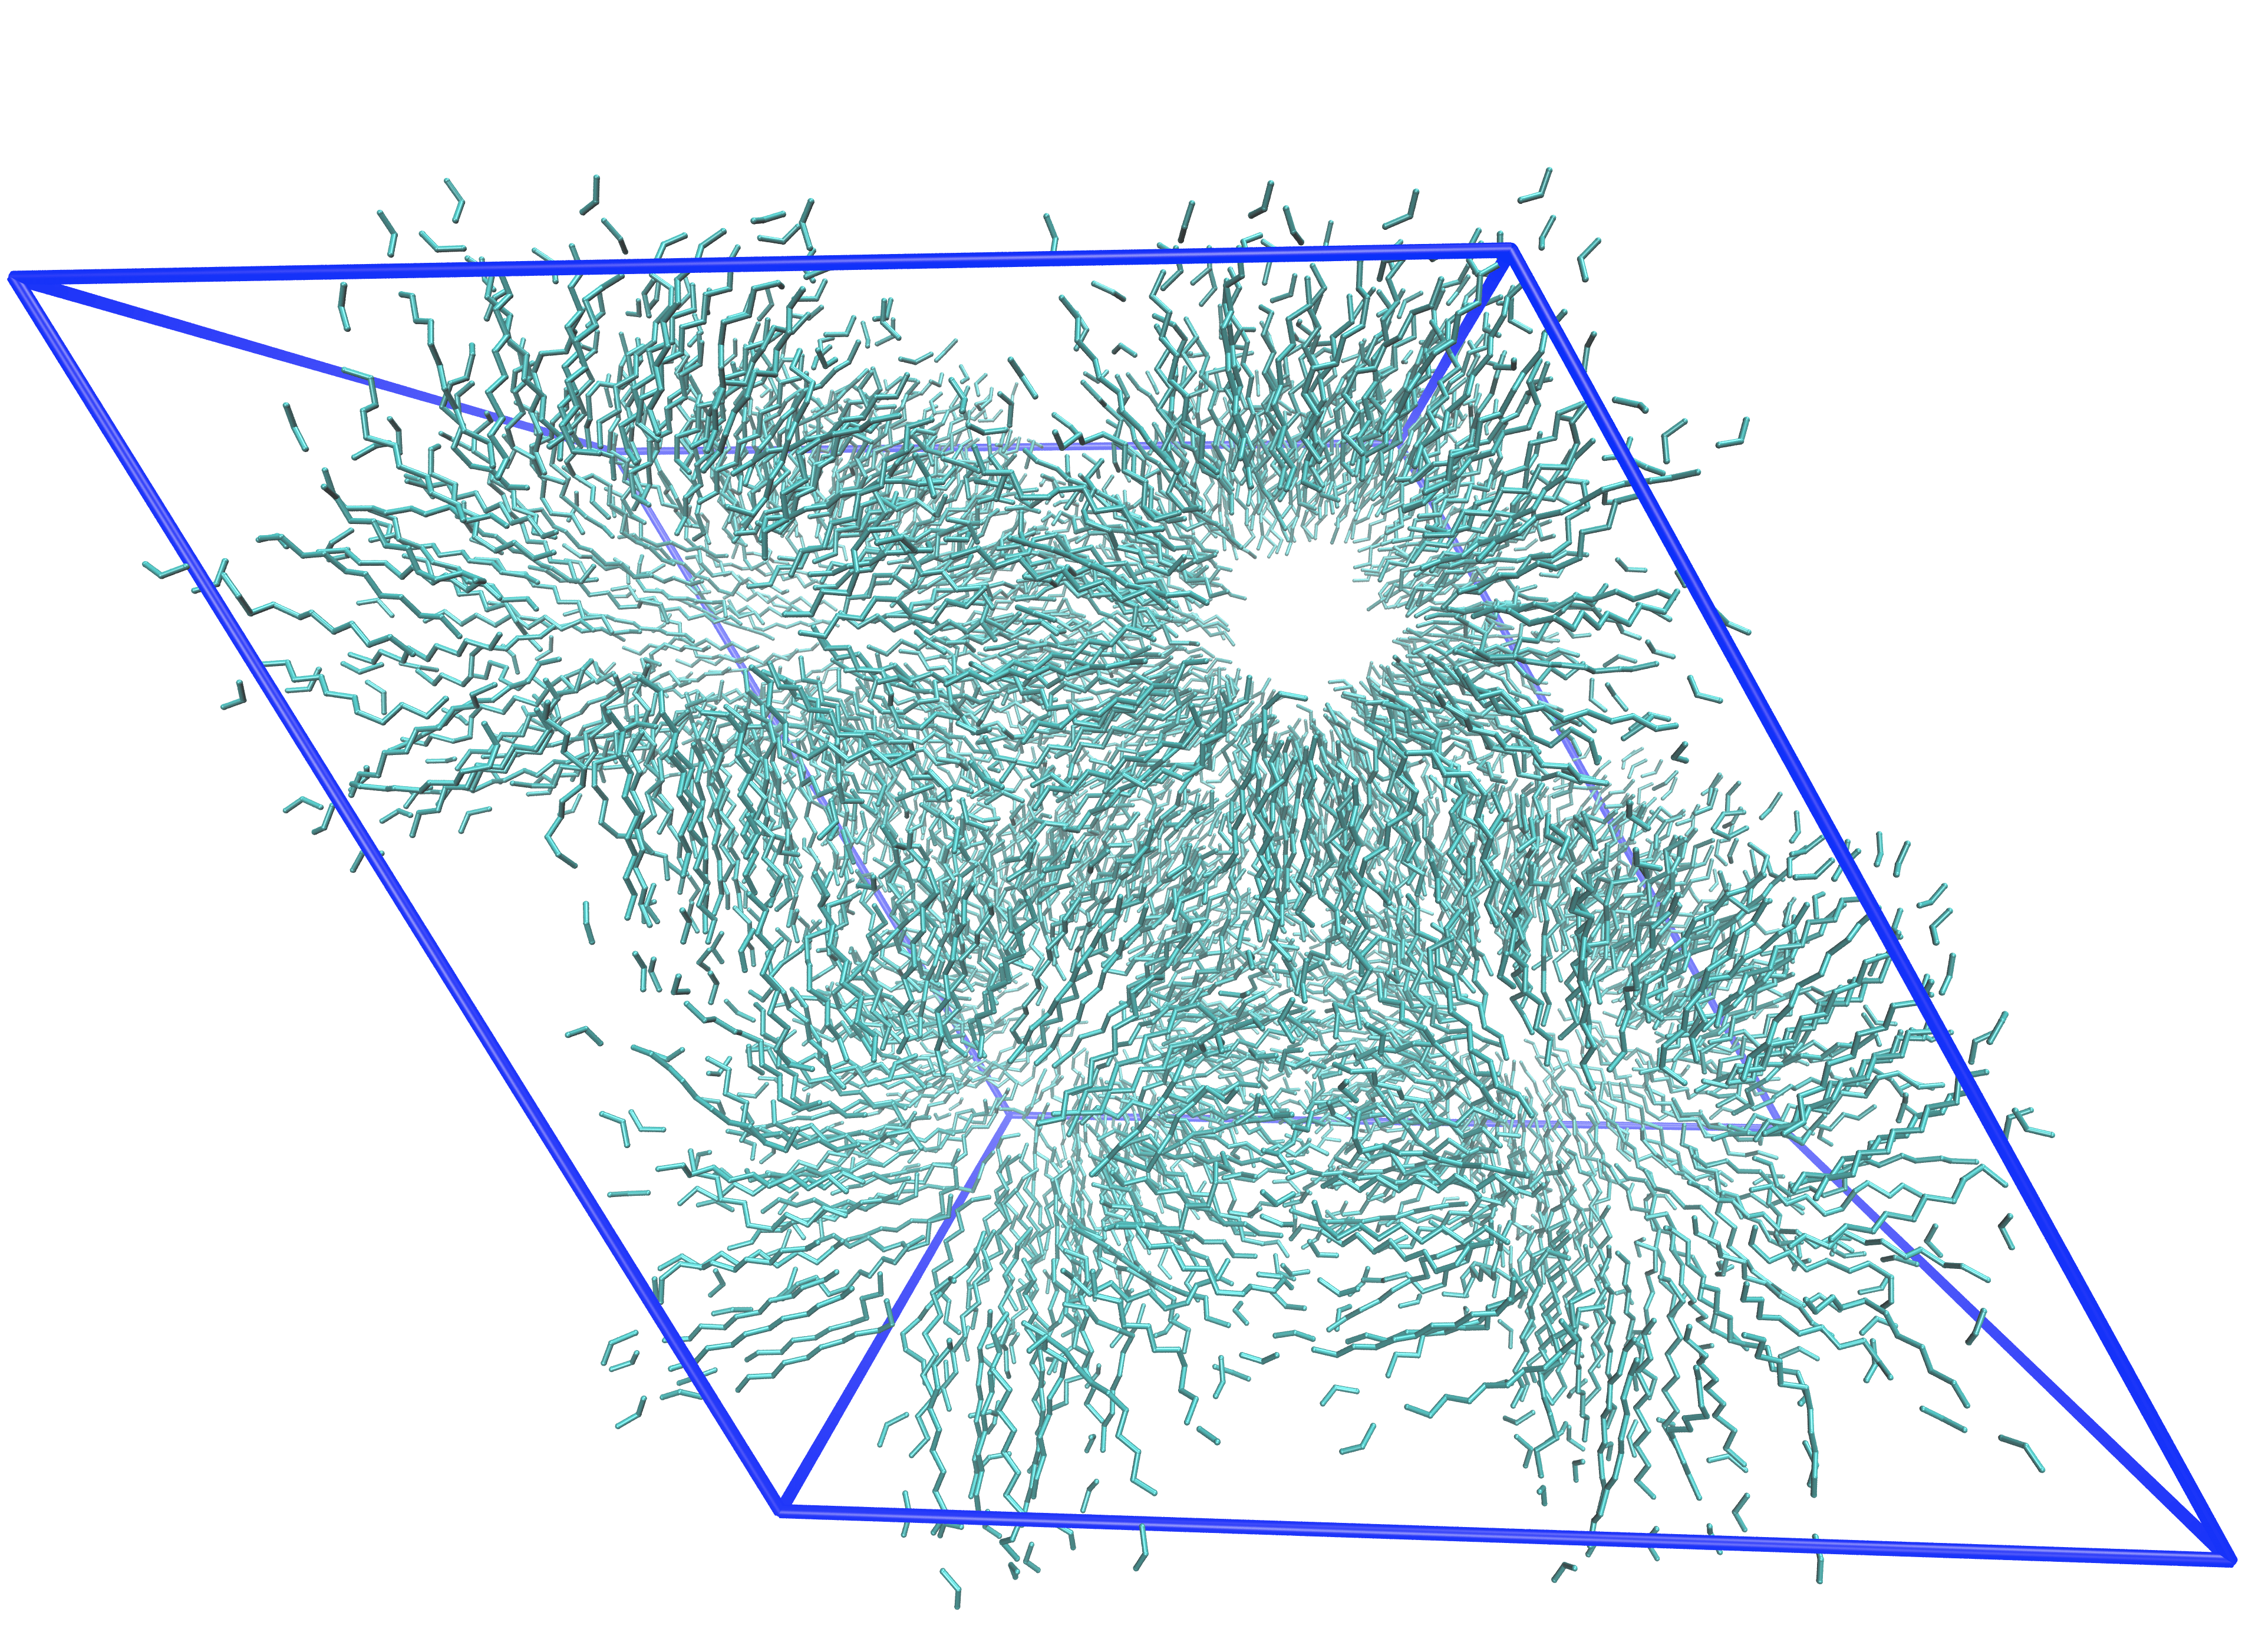
\includegraphics[width=\textwidth,scale=2]{tails_topview.png}
                \caption{}\label{fig:tails_topview}
        \end{subfigure}
        \begin{subfigure}{0.45\textwidth}
                \centering
                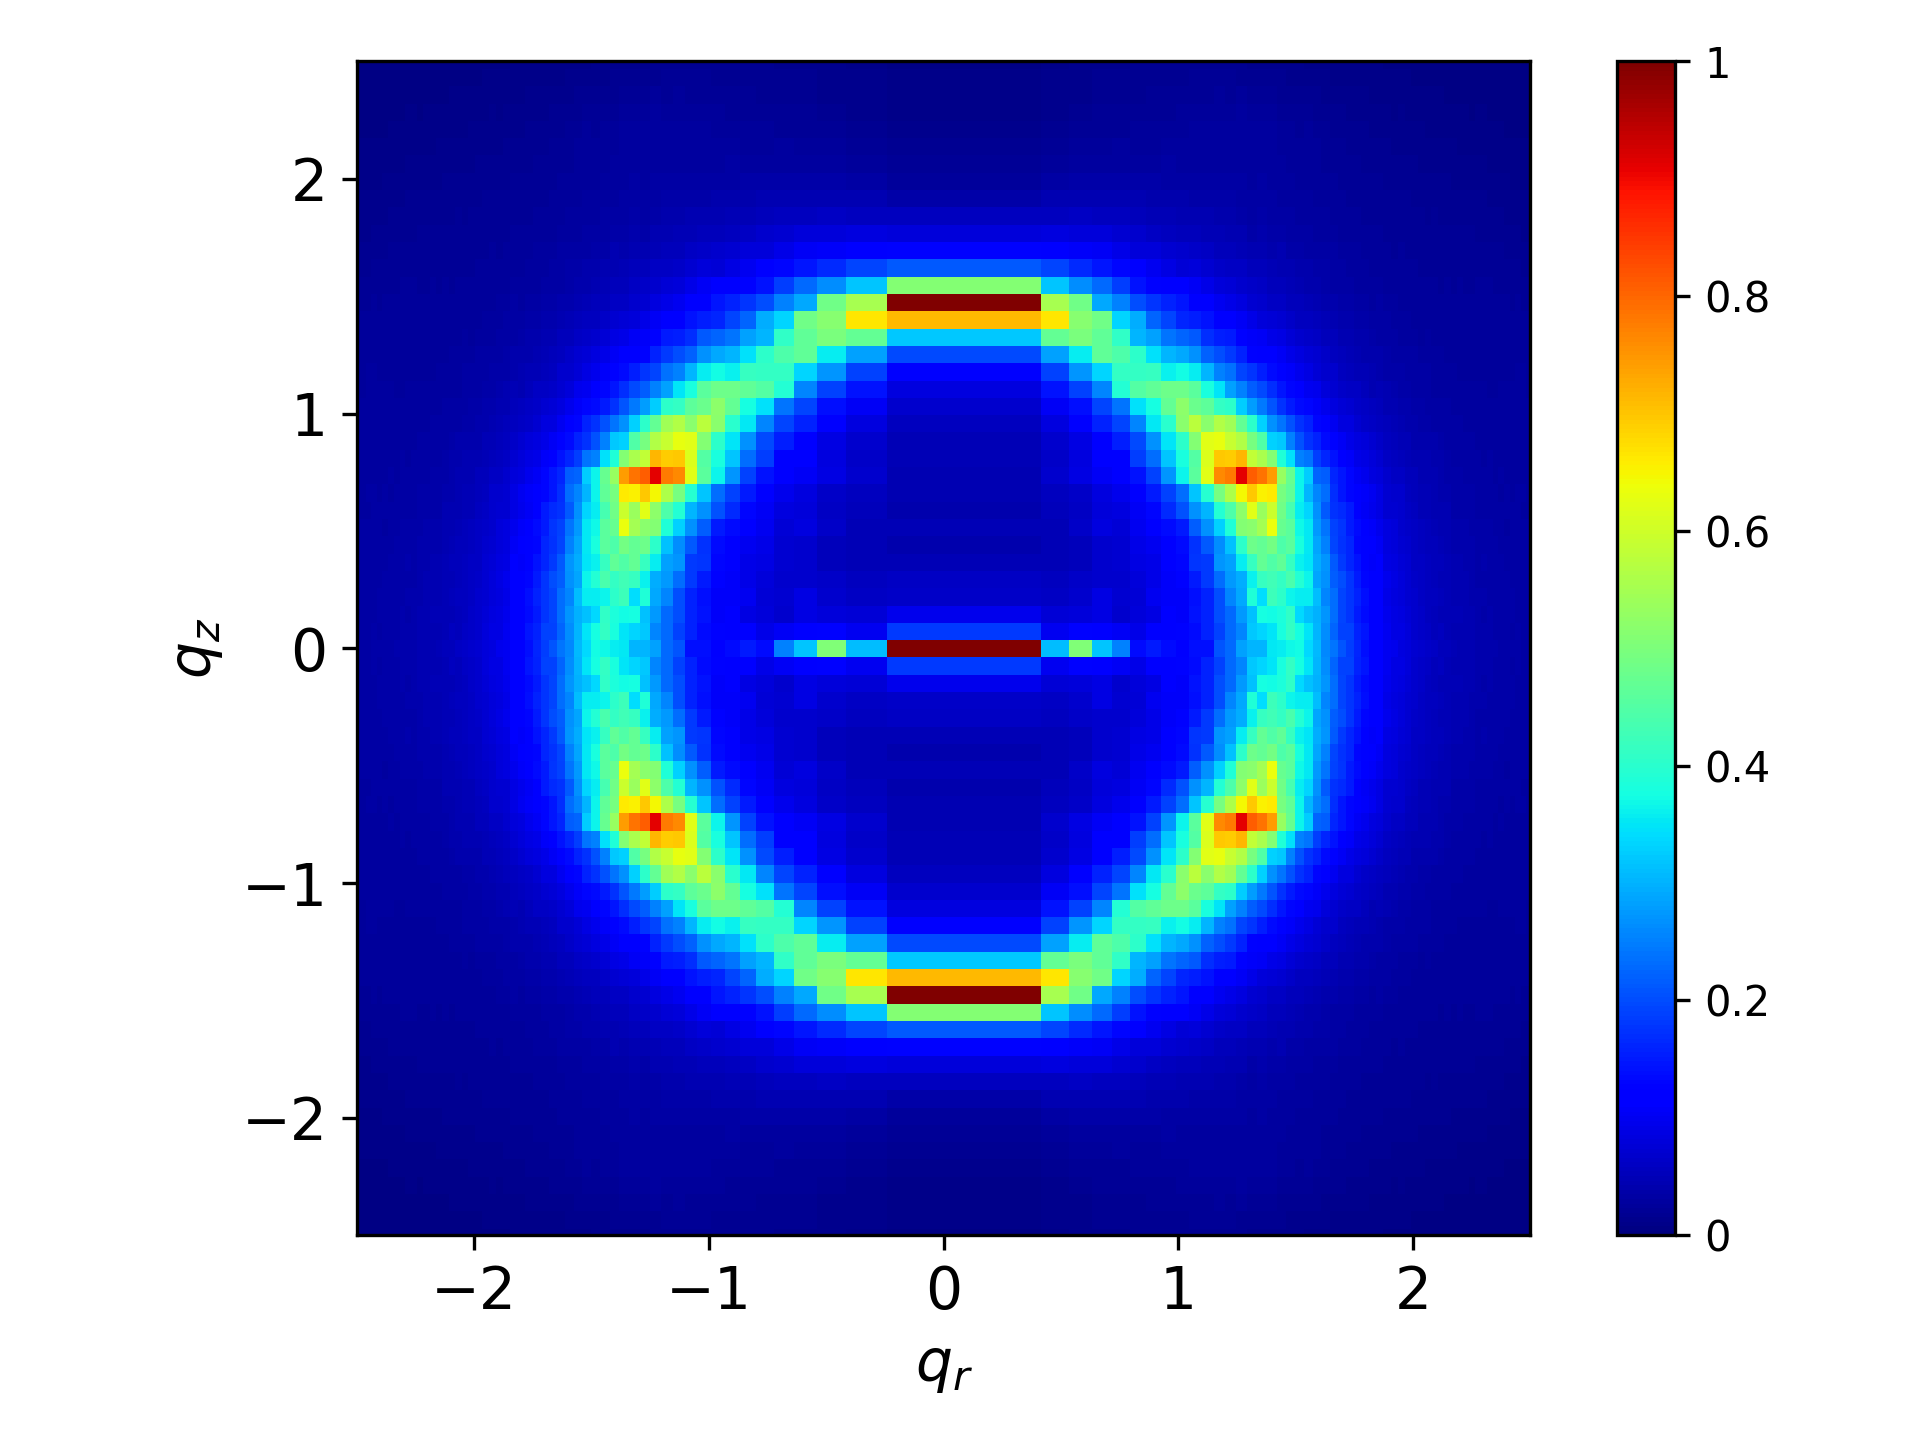
\includegraphics[width=\textwidth]{tails_rzplot.png}
                \caption{}\label{fig:tails_rzplot}
        \end{subfigure}
        \begin{subfigure}{0.45\textwidth}
                \centering
                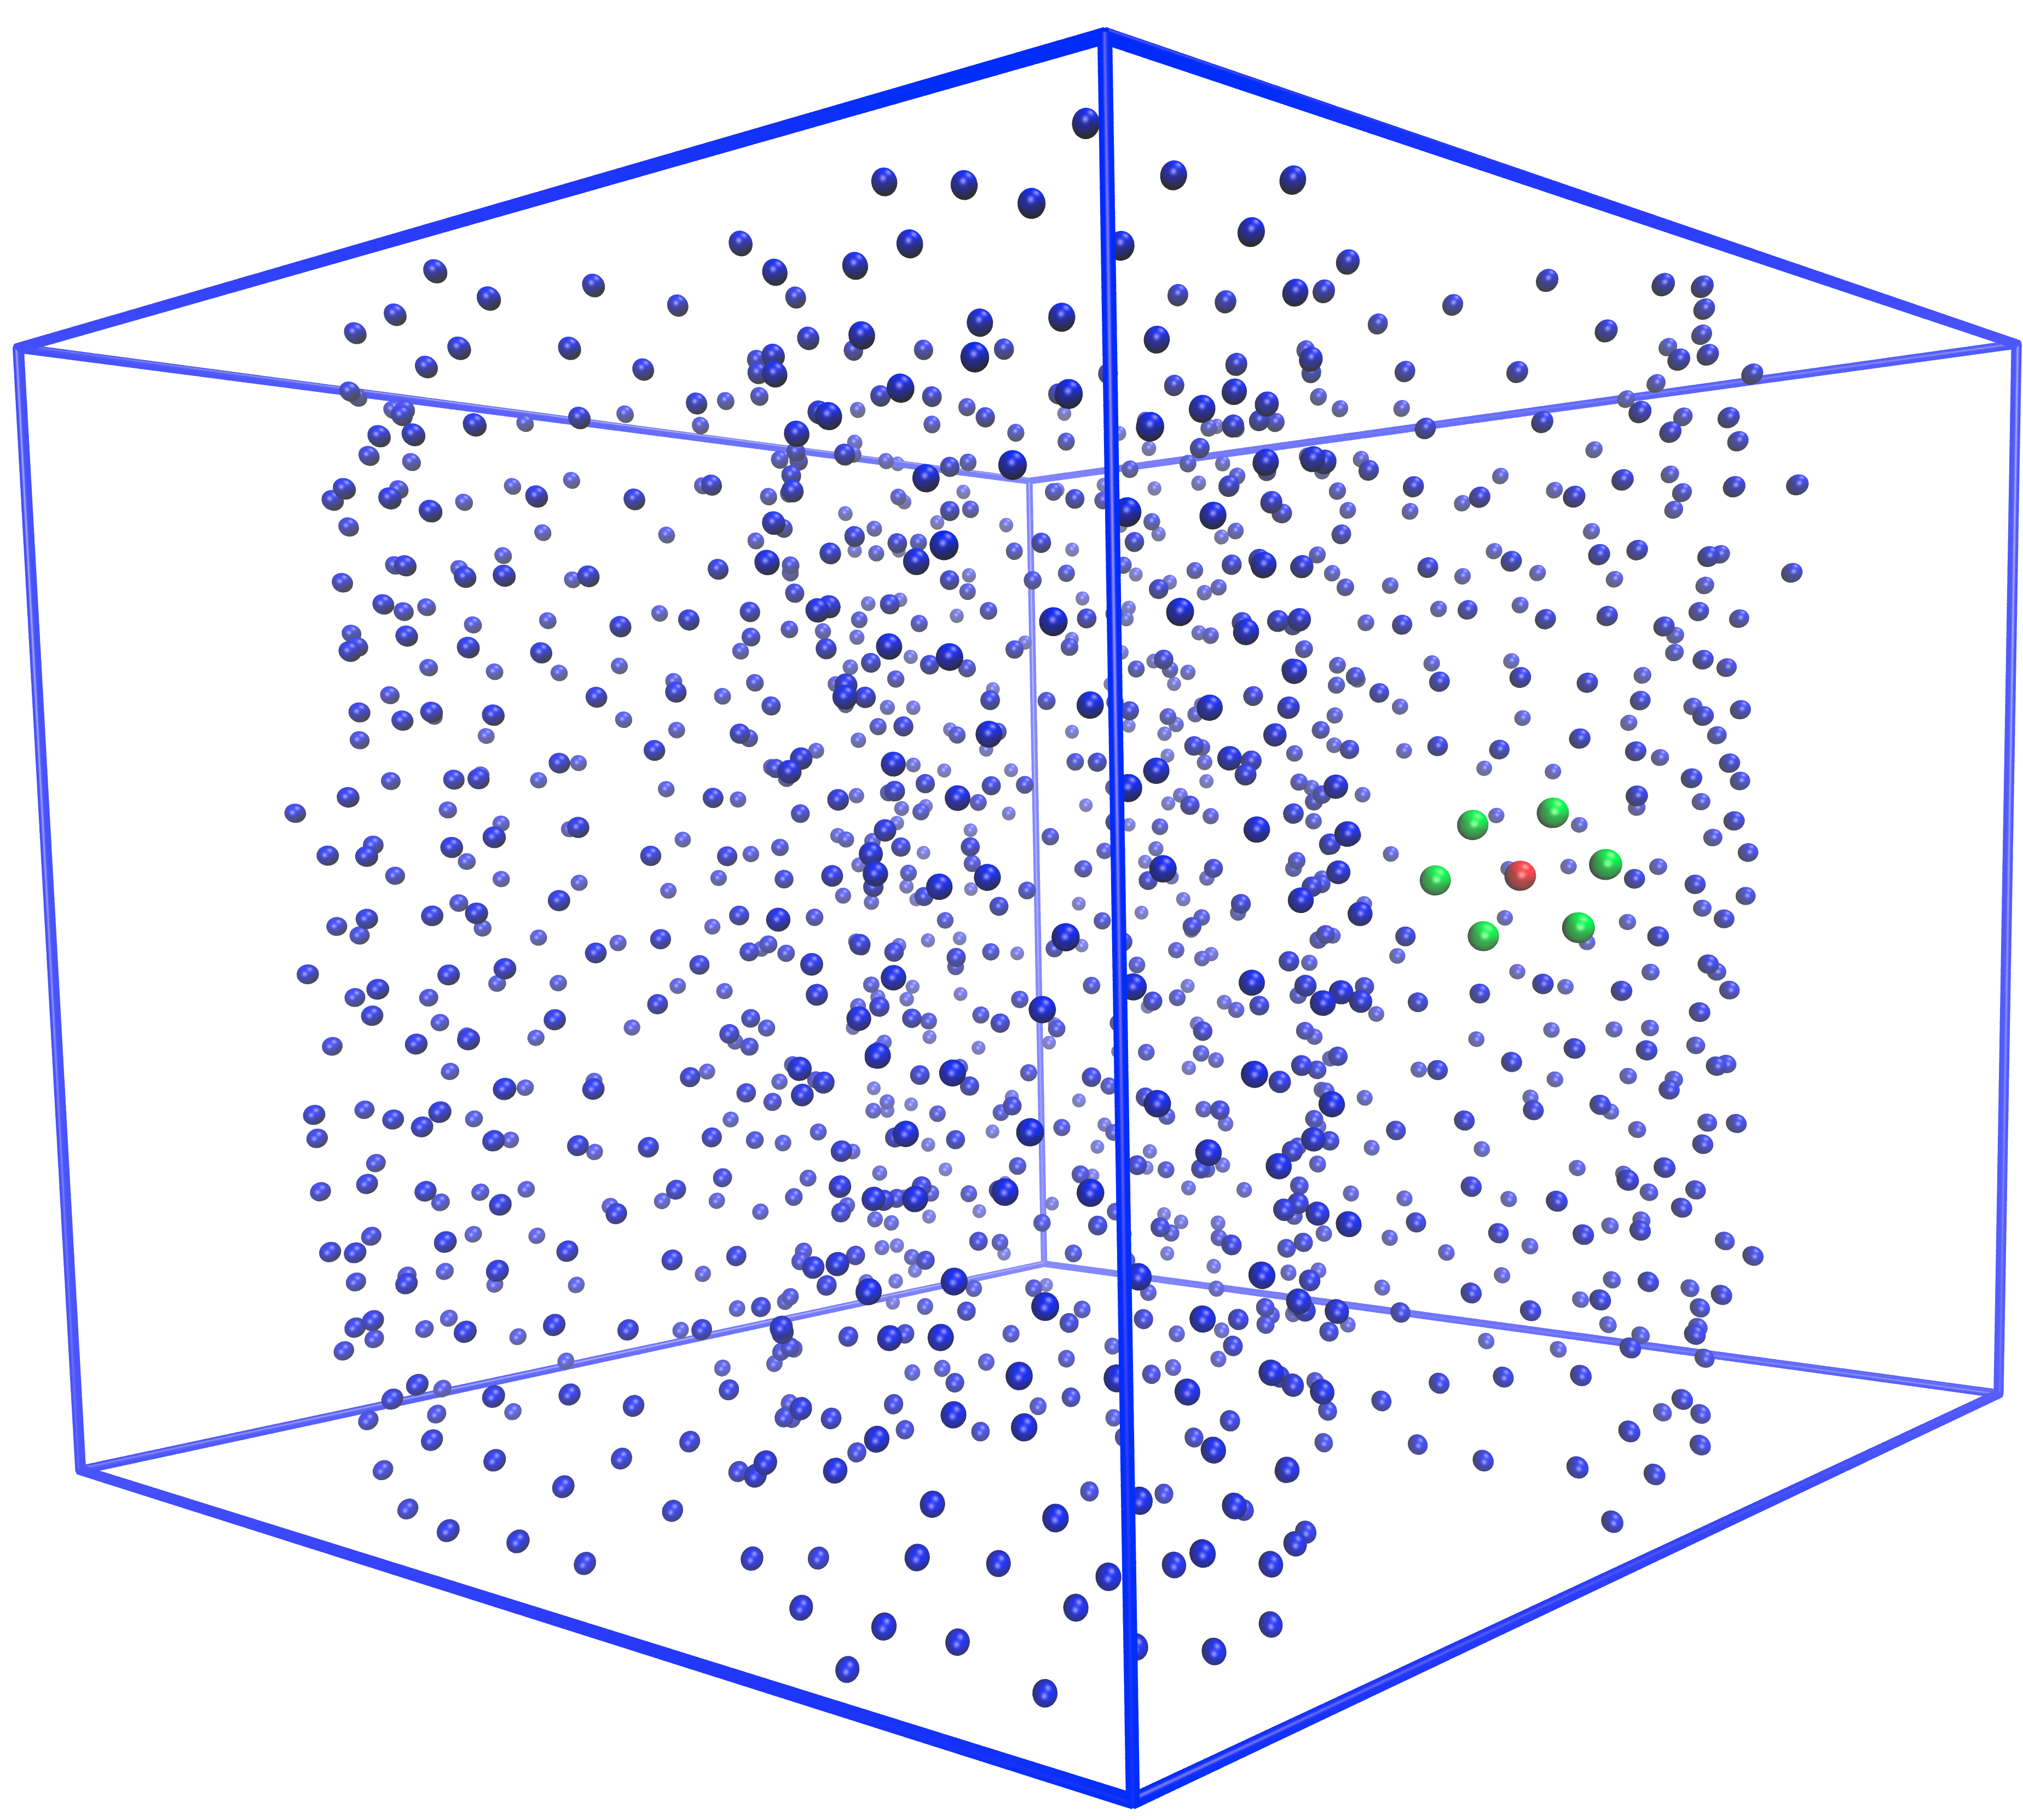
\includegraphics[width=\textwidth]{centroids_box.png}
                \caption{}\label{fig:centroids}
        \end{subfigure}
        \begin{subfigure}{0.45\textwidth}
                \centering
                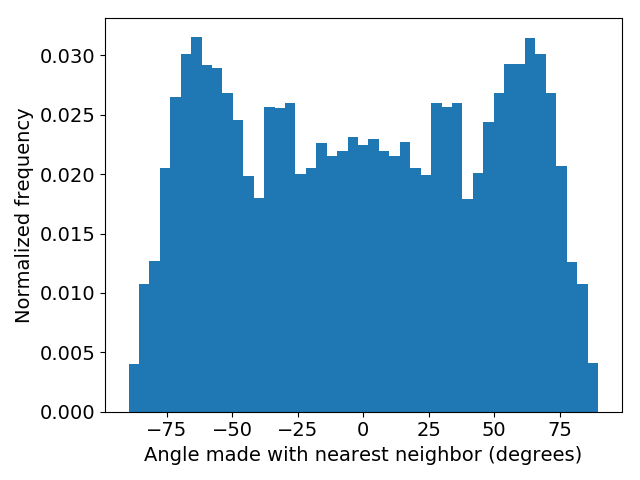
\includegraphics[width=\textwidth]{angles_traj_layered.png}
                \caption{}\label{fig:angle_distribution}
        \end{subfigure}
        \caption{(a) The trajectory can be stripped of all atoms except carbon
        atoms in monomer tails. (b) Simulated diffraction of the tail-only trajectory
        still gives rise to R-spots. (c) Finding the center of mass and visualizing
        their coordinates reveals the hexagonal-like packing of the tails. (d) The
        distribution created by measuring the angle between each centroid (e.g. red
        in (c)) and its neareset neighbors (e.g. green in (c)) with respect to the xy
        plane has distinct spikes near 30\degree, which is consistent with the location
        of R-spots}\label{fig:tail_packing}
\end{figure}



\end{document}
